% aspectratio: 43 for old style 4:3, 169 for wide screen 16:9
% If you don't know if the screen will be wide screen or 4:3 you can use
% 1610 for a compromise to have smaller borders on either of the usual aspect ratios
% \documentclass[aspectratio=169,9pt]{beamer}
\documentclass[
aspectratio=169,
14pt,
professionalfonts
]{beamer}

\usetheme[patchframe=true]{LMU}
% \usepackage{fontspec}
% \setsansfont{Source Sans Pro}
% \setmonofont{Fira Code}[Contextuals=Alternate]

% \usepackage{mathspec}

\renewcommand*{\thefootnote}{\fnsymbol{footnote}}

\newcommand\identity{1\kern-0.25em\text{l}}

\newcommand{\pyhf}{\texttt{pyhf}\xspace}

\newcommand{\arrow}{~\ding{220}~}

\DeclareMathOperator\supp{supp}

\title[]{Illuminating the dark side of statistics: \\ Bayesian inference in particle physics}

\author[L. G\"artner]{\underline{Lorenz G\"artner}$^{1}$}

\institute[LMU]{$^1$LMU Munich}

\date{\today}

\begin{document}
%TODO references

\begin{frame}[titleslide]
    \titlepage
    \begin{tikzpicture}[remember picture,overlay]
    \node[anchor=south west, yshift=2mm, xshift=2mm] at (current page.south west)
    {%
      
\includegraphics[height=1.cm]{common/logos/origins.pdf}
      
\includegraphics[height=1.cm]{common/logos/belle2.pdf}
      
\includegraphics[height=1.cm]{common/logos/punch4nfdi.png}
      
\includegraphics[height=1.cm]{common/logos/dfg.jpg}
      % 
\includegraphics[height=1.5cm]{common/logos/bmbf.pdf}
    };%
    \end{tikzpicture}
\end{frame}

\begin{frame}{About me}
    \begin{minipage}{0.69\textwidth}
        \begin{itemize}
            \item BSc @ University of Manchester \\
                Physics with theoretical physics\\
                Little stats
            \item MSc @ LMU Munich \\
                Thesis on QFT in curved spacetime\\
                Almost no stats
            \item Currenly PhD @ LMU Munich\\
                A lot of stats
        \end{itemize}
    \end{minipage}
    \begin{minipage}{0.3\textwidth}
        \begin{figure}
            \center
            
\includegraphics[width=\textwidth]{../plots/port.jpg}
        \end{figure}
    \end{minipage}
\end{frame}

\begin{frame}
\centering
\Large
What is a probability?
\end{frame}

\begin{frame}{Kolmogorov probability axioms}
% https://plato.stanford.edu/entries/probability-interpret/#MaiInt
\begin{enumerate}
  \item $ p(\Omega) = 1 $, where \( \Omega \) is the sample space.
  \item $ p(x) \geq 0 $ for any event \( x \subseteq \Omega \).
  \item For any sequence of disjoint events \( x_1, x_2, \dots \),
        $$
        p\left( \bigcup_{i=1} x_i \right) = \sum_{i=1} p(x_i)
        $$
\end{enumerate}
\end{frame}


\begin{frame}{Conditional probability}
Is \textbf{defined} as the probability of an event $x$ if we know that an event $y$ is true $p(x|y)$.
$$p(x \cap y) = p(x|y)p(y) \quad \to \quad p(x|y) = \frac{p(x \cap y)}{p(y)}$$

\textit{Note} 
$$p(x \cap y) = p(y \cap x) \quad  \text{but} \quad p(x|y) \neq p(x|y)$$ 
\end{frame}

\begin{frame}{Probability interpretations}
    Axioms:
    \begin{center}
        old probabilities \arrow new probabilities
    \end{center}
    
    \vspace{0.5cm}
    To assign probabilities we need probability interpretations.

    \vspace{0.5cm}
    The interpretations \textbf{share the same mathematical framework}, but the meaning of $p(x)$ is different.
\end{frame}

\begin{frame}{Frequentist interpretation}
    Assign a probability as relative frequency
    \begin{minipage}{0.60\textwidth}
        $$
        p(x) = \lim_{N\to\infty} \frac{N_x}{N}
        $$

        \begin{itemize}
            \item "The data is random."
            \item Repeatable experiments only
            \item $p(x)$ for $N=1$?
        \end{itemize}
    \end{minipage}
    \begin{minipage}{0.39\textwidth}
        \begin{figure}
            \centering
            
\includegraphics[width=\textwidth]{../plots/die-title.png}
            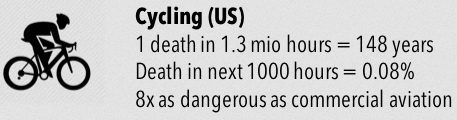
\includegraphics[width=\textwidth]{../plots/die-bike.png}
            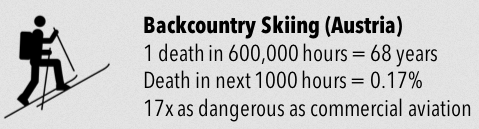
\includegraphics[width=\textwidth]{../plots/die-ski.png}
            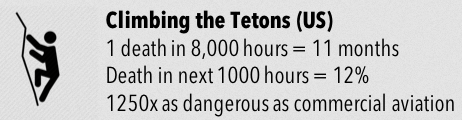
\includegraphics[width=\textwidth]{../plots/die-climbing.png}
        \end{figure}
        %https://chessintheair.com/the-risk-of-dying-doing-what-we-love/
    \end{minipage}
\end{frame}

\begin{frame}{Bayesian interpretation}
    Assign a probability $p(x)$ as \textit{degree of belief}.
    \begin{itemize}
        \item "Parameters are random".
        % \item Probability depends on the experimenters' knowledge.
        \item Inference results are subjective.
    \end{itemize}
        \begin{figure}
            \centering
            
\includegraphics[width=0.4\textwidth]{../plots/die-title.png}\\
            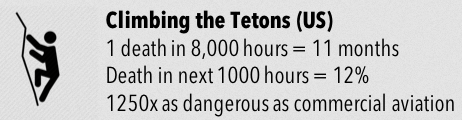
\includegraphics[width=0.4\textwidth]{../plots/die-climbing.png}
        \end{figure}
        $$p(death|experienced) \neq p(death|unexperienced)$$
        %https://chessintheair.com/the-risk-of-dying-doing-what-we-love/
\end{frame}

\begin{frame}{Bayes' theorem}

The \textbf{posterior} is

$$
\tcbhighmath[colback=yellow]{
p(\text{theory} | \text{data}) = \frac{p(\text{data}|\text{theory}) p(\text{theory})}{p(\text{data})}
}
$$

\begin{itemize}
    \item \textbf{Likelihood} $p(\text{data}|\text{theory})$
    \item \textbf{Prior} $p(\text{theory})$
    \item \textbf{Evidence} $p(\text{data}) = \int p(\text{data}|\text{theory}) p(\text{theory})$
\end{itemize}
\begin{flushright}
    \textit{Can you derive it?}
\end{flushright}
\end{frame}

\begin{frame}
    \textit{ [...] nearly all physicists tend to misinterpret frequentist results as statements about the theory given with the data.}\\
    \flushright Presentation of search results: the $CL_s$ technique,\\ A. L. Read
\end{frame}

\begin{frame}{The common ground}
    \textbf{Frequentist inference} is based on 
    $$\tcbhighmath[colback=yellow]{p(x|\theta)}$$
    \textbf{Bayesian inference} is based on
    $$p(\theta | x) = \frac{\tcbhighmath[colback=yellow]{p(x|\theta)} p(\theta)}{p(x)}$$
    \arrow \textbf{You want the best possible $\tcbhighmath[colback=yellow]{p(x|\theta)}$.}
\end{frame}

\begin{frame}[noframenumbering]{The best possible model...}
    \begin{figure}
        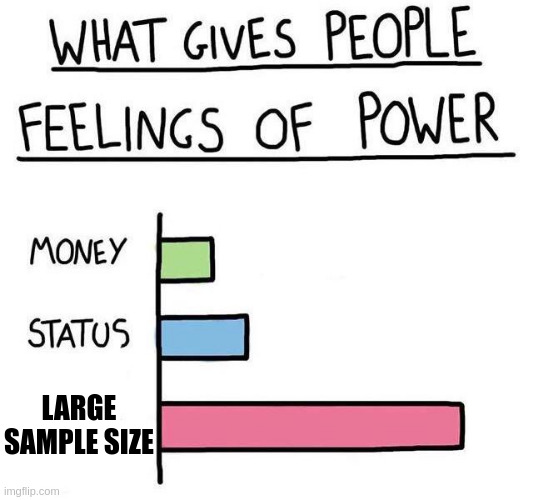
\includegraphics[width=0.4\textwidth]{../plots/sample_size.jpg}
    \end{figure}
\end{frame}

\begin{frame}{Physics does not care...}{... about our interpretation}
For many inference problems, the frequentist and Bayesian approaches give similar numerical values, even though they answer different questions.

\vspace{0.5cm}

BUT if results are different, you should understand why.
\end{frame}

\begin{frame}
\center
\Large
Parameter inference
\end{frame}

\begin{frame}{Parameter inference}
    \center
    \textbf{Point estimates}\\
    Identify the most probable parameter point.

    \vspace{1cm}

    \textbf{Interval estimation}\\
    Identify extended regions in parameter space based on compatibility with the data.
\end{frame}

\begin{frame}{Frequentist point estimates: estimators}
    Estimator is a \textit{statistic} $\hat \theta(x)$, with desired properties
    \begin{minipage}{0.65\textwidth}
        \begin{itemize}
            \item \textbf{consistency}\\
            $\lim_{n_x \to \infty} E_x[\hat \theta] = \theta_{true}$
            % converges toward true value as number of observations increase
            \item \textbf{unbiasedness}\\
            $b = E_x[\hat \theta] - \theta_{true}$
            
            \item \textbf{efficiency}\\
            $V(\hat \theta) = I(\theta)^{-1} = E_x\left[\left(\frac{\partial \ln p(x|\theta)}{\partial \theta}\right)^2\right]^{-1}$
            % minimum variance
            \item ...
        \end{itemize}
    \end{minipage}
    \begin{minipage}{0.34\textwidth}
        \begin{figure}
            \centering
            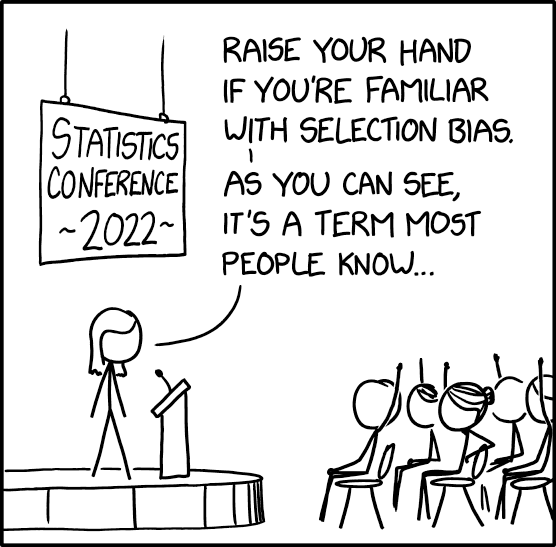
\includegraphics[width=\linewidth]{../plots/selection_bias_2x.png}
        \end{figure}
    \end{minipage}
\end{frame}

\begin{frame}{A good data set is the key to success ...}
    \begin{figure}
    \centering
    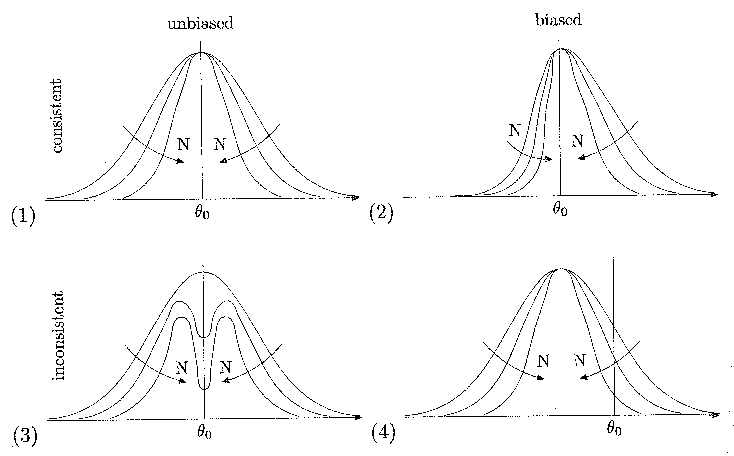
\includegraphics[width=0.8\linewidth]{../plots/estimator.pdf}
\end{figure}
\end{frame}

\begin{frame}{Method of maximum likelihood}
    \vspace{-0.2cm}
    We find maximum likelihood estimators $ \hat \theta$ by solving
    $$\hat \theta = \text{argmax}_\theta ~ p(x|\theta)$$
    It has the property
    $$
    \lim_{N \to \infty} p\left(\sqrt{N}(\hat \theta - \theta_{true})\right) = \mathcal{N}\left(0, I^{-1}(\theta)\right),
    $$
    implying consistency, asymptotic unbiasedness and efficiency.
    % $$ \lim_{N \to \infty} V(\hat \theta) = I(\theta)^{-1} = E\left[\frac{\partial \ln p(x|\theta)}{\partial \theta}\right]^{-1}$$
\end{frame}

% \begin{frame}{Asymptotic normality}
%     In the asymptotic limit $N \to \infty$ they have the properties of
%     $$
%     lim_{N_x \to \infty} \sqrt{N}(\hat \theta - \theta_{true}) \sim \mathcal{N}(0, I^{-1}(\theta))
%     $$
%     \begin{itemize}
%         \item \textit{consistency}
%         \item \textit{efficiency}: variance given by Cramer-Rao bound
%         $$ \lim_{N_x \to \infty} V(\hat \theta) = E\left[\frac{\partial \ln L(x|\theta)}{\partial \theta}\right]^{-1}$$
%         \item \textit{robustness}: asymptotically Normal
%     \end{itemize}
% \end{frame}

\begin{frame}{Bayesian point estimates}
    \begin{minipage}{0.49\textwidth}
        \textbf{Mode}\\ Value of $\theta$ with maximum a-posteriori probability
            $$\theta^* = \text{argmax}_\theta ~ p(\theta|x)$$
        \textbf{Mean}\\ Expected value of $\theta$ under the posterior
            $$ \bar{\theta} = E_{p(\theta|x)}[\theta]$$
    \end{minipage}
    \begin{minipage}{0.49\textwidth}
        \begin{figure}
            \centering
            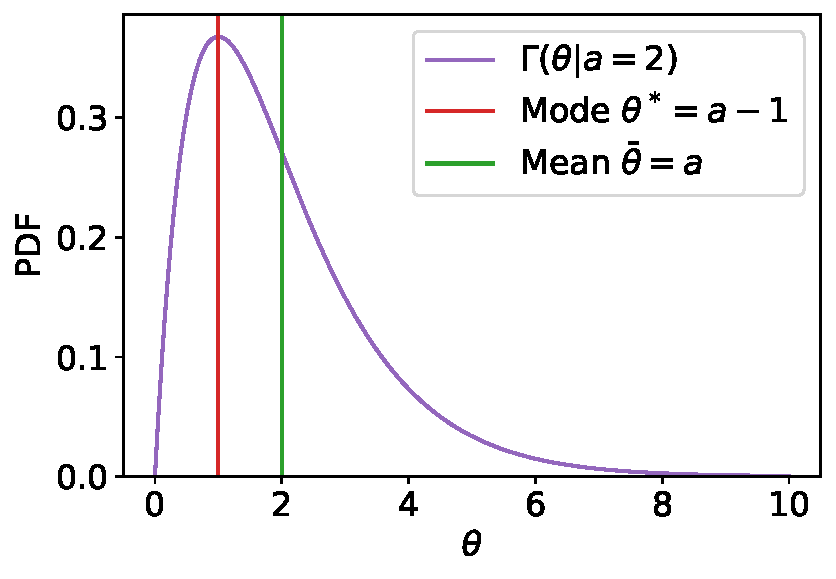
\includegraphics[width=\linewidth]{../plots/map_vs_mean.pdf}
        \end{figure}
    \end{minipage}
\end{frame}

\begin{frame}{Bayesian point estimates}
        \textbf{Mode}\\ Value of $\theta$ with maximum a-posteriori probability
            $$\theta^* = \text{argmax}_\theta ~ p(\theta|x)$$
        \textit{Note}
        $$\frac{\partial p(\theta|x)}{\partial \theta}\bigg\vert_{\theta = \theta^*} \propto 
        \left(
            \frac{\partial p(x|\theta)}{\partial \theta}p(\theta) + p(x|\theta) \frac{\partial p(\theta)}{\partial \theta}\right)\bigg\vert_{\theta = \theta^*} = 0$$
        $$\implies \theta^* = \hat \theta \quad \textrm{if} \quad \frac{\partial p(\theta)}{\partial \theta}\bigg\vert_{\theta = \theta^*}=0$$
\end{frame}

\begin{frame}{Intervals and limits}
\begin{figure}
    \centering
    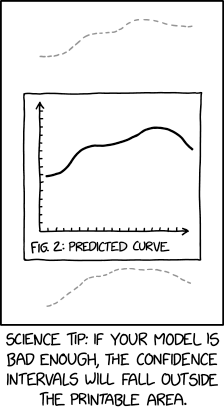
\includegraphics[width=0.25\linewidth]{../plots/confidence_interval.png}
    %https://xkcd.com/2311
\end{figure}
\end{frame}

\begin{frame}{Intervals and limits}
If an estimator PDF is not Normal, $\hat \theta \pm \sigma_\theta$ is meaningless.

\begin{figure}
    \centering
    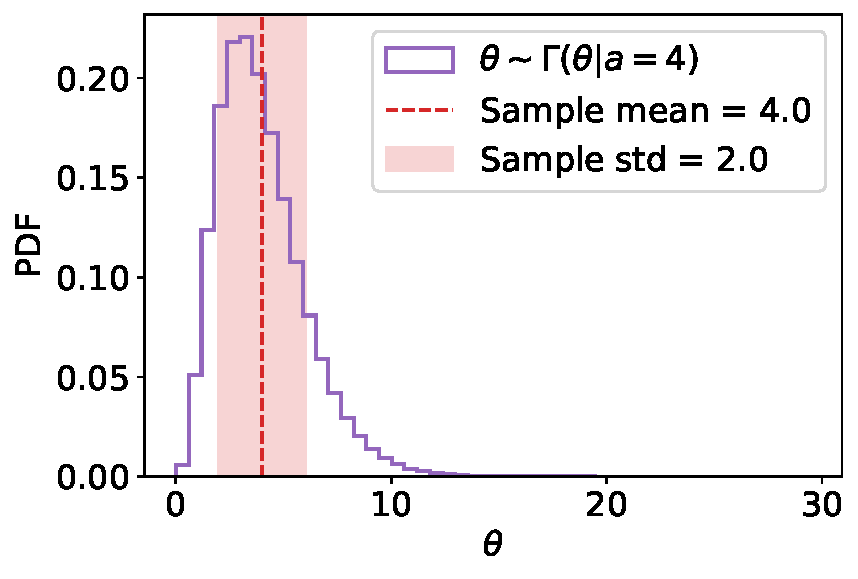
\includegraphics[width=0.6\linewidth]{../plots/gamma.pdf}
\end{figure}
\end{frame}

\begin{frame}{Frequentist intervals}

\begin{minipage}[t]{0.55\linewidth}
\textbf{Neyman confidence belt}
$$
\int_{x_1}^{x_2} dx ~ p(x|\theta) = 1-\alpha
$$
Not unique \arrow \textit{central interval}
\small
$$
\int_{-\infty}^{x_1} dx ~ p(x|\theta)=  \int_{x_2}^{\infty} dx ~ p(x|\theta) = \alpha/2
$$
\normalsize
or \textit{upper/lower interval}
\end{minipage}
\begin{minipage}[t]{0.44\linewidth}
    \begin{figure}
        \centering
        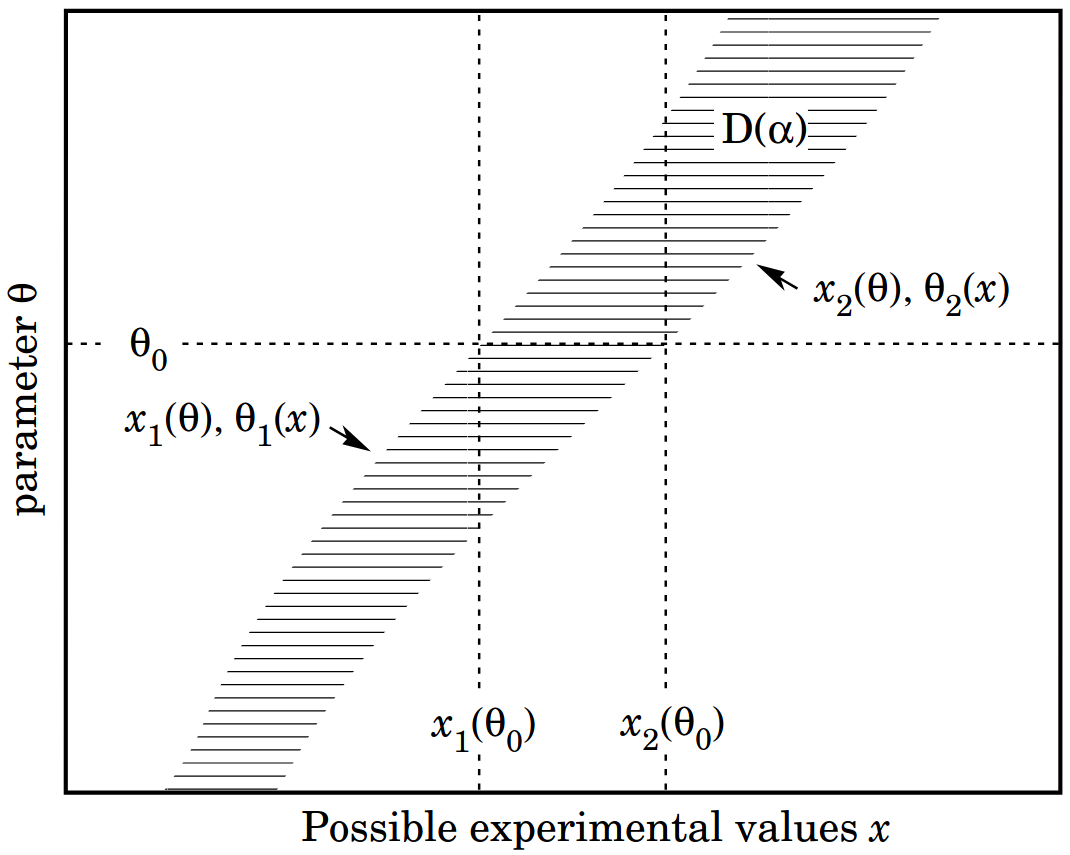
\includegraphics[width=\linewidth]{../plots/neyman.png}
    \end{figure}
\end{minipage}
\end{frame}

\begin{frame}{Bayesian intervals}

Credible intervals $[\theta_1, \theta_2]$ cover $1-\alpha$ of the posterior
$$
\int_{\theta_1}^{\theta_2} d\theta ~ p(\theta| x) = 1-\alpha
$$
\begin{itemize}
    \item For upper/lower limits: set $\theta_1$ or $\theta_2$ to boundary
    \item \textit{Smallest possible interval}\\
        \arrow Highest (posterior) density intervals (HDI)
\end{itemize}
\end{frame}

\begin{frame}{$b\to u l^- \bar \nu$ in the Weak Effective Theory}
    \vspace{-0.5cm}
    \begin{minipage}{0.5\textwidth}
        \begin{figure}
            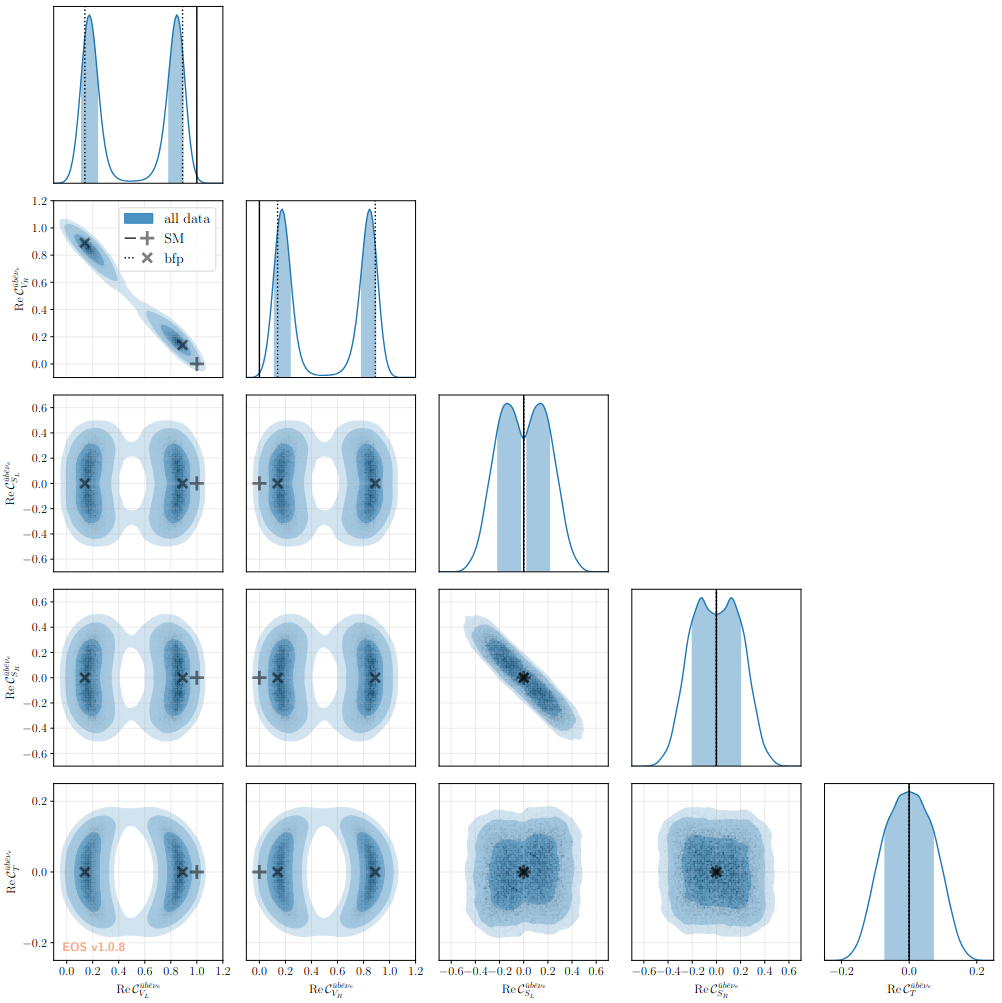
\includegraphics[width=\textwidth]{../plots/wet-posterior.png}
        \end{figure}
    \end{minipage}
    \begin{minipage}{0.49\textwidth}
        \begin{itemize}
            \item \href{https://corner.readthedocs.io/en/latest/}{Corner plots} are great for visualization.
            \item Marginal posterior for Wilson coefficients
            \item Identify modes, credible intervals
            \item Best fit point $\neq$ mode, why?
        \end{itemize}
        \vspace{0.5cm}
        \begin{flushright}
            \href{https://arxiv.org/pdf/2302.05268}{arXiv:2302.05268v2 [hep-ph]}
        \end{flushright}
    \end{minipage}
\end{frame}

\begin{frame}
    \center
    \Large
    Nuisance parameters and priors
    \end{frame}
    
    \begin{frame}{Nuisance parameters}

        \begin{minipage}{0.49\textwidth}
            Models are not perfect \\
            \arrow \textbf{systematic bias}

            \vspace{0.5cm}
            \textit{Solution}: \\
            \textbf{Nuisance} parameters $\nu$,
            $$p(x|\psi, \nu)$$
        \end{minipage}
        \begin{minipage}{0.49\textwidth}
            \begin{figure}
                \centering
                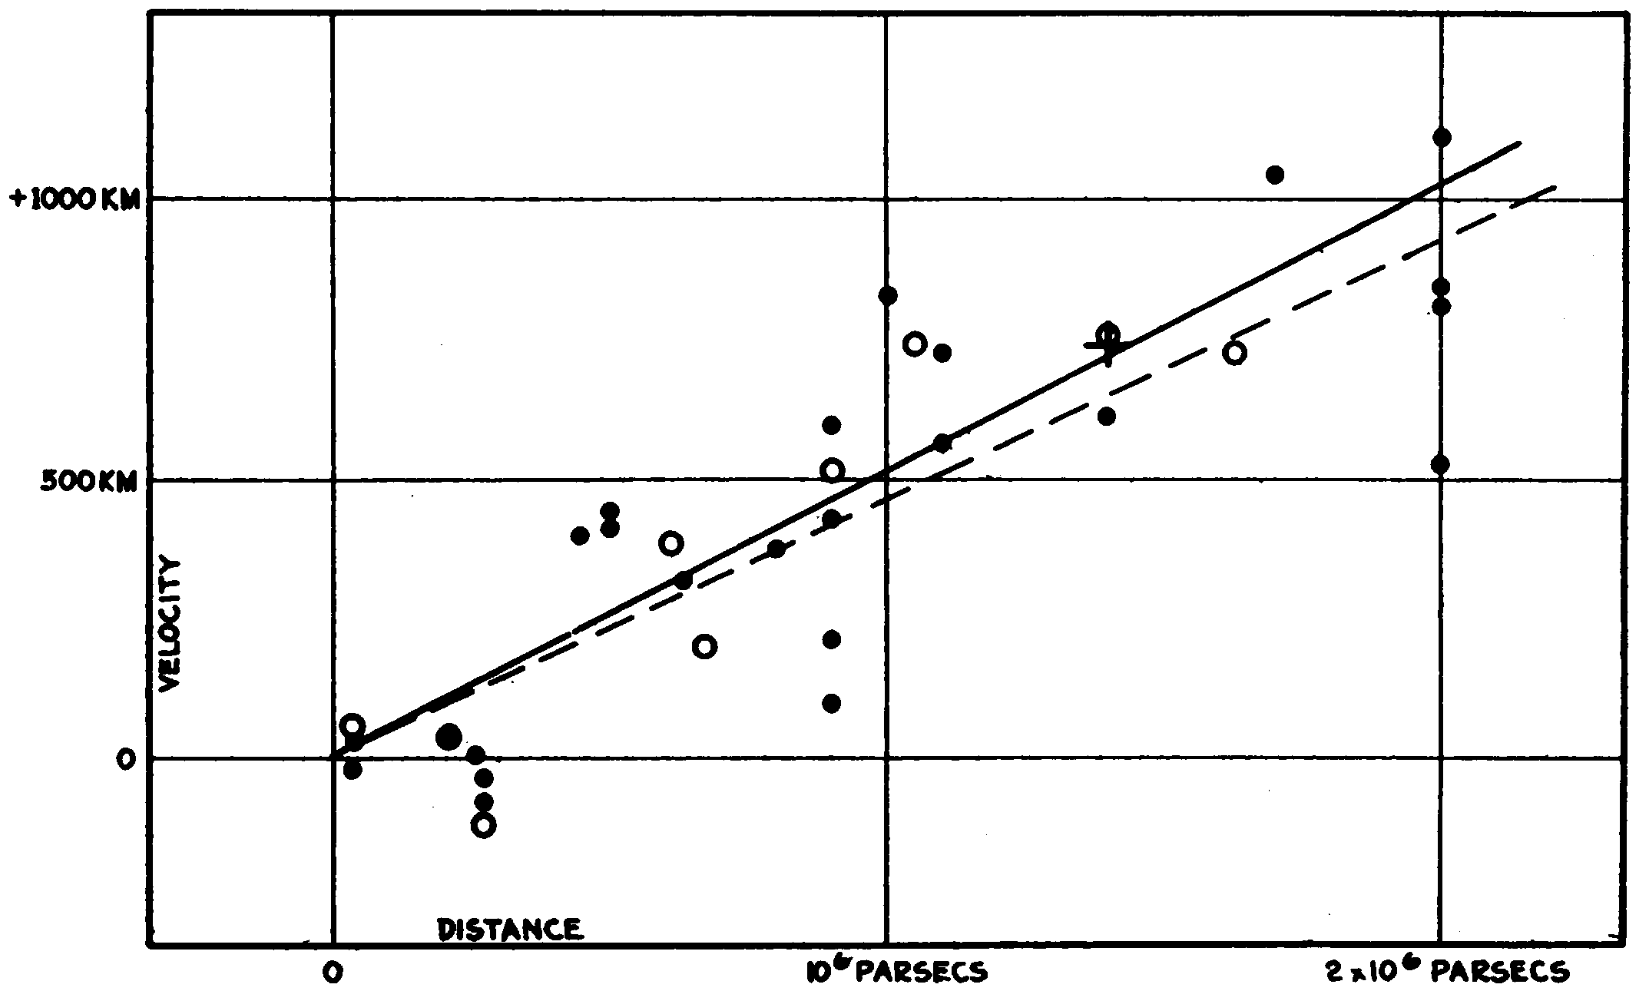
\includegraphics[width=\textwidth]{../plots/hubble.png}
            \end{figure}
            \flushright \small
            \href{https://www.pnas.org/doi/10.1073/pnas.15.3.168}{Hubble 1929}
        \end{minipage}
    \vspace{0.5cm}
    % In general the model is not perfect, which is to say it cannot provide an accurate description of the data even at the most optimal point of its parameter space. As a result, the estimated parameters can have a systematic bias.
    
    % Although including additional parameters may eliminate or at least reduce the effect of systematic uncertainties, their presence will result in increased statistical uncertainties for the parameters of interest. This occurs because the estimators for the nuisance parameters and those of interest will in general be correlated.
    
    Usually, we want to constrain nuisance parameters, but in the frequentist language \textbf{everything is data}.
    % To reduce the impact of the nuisance parameters one often tries to constrain their values by means of control or calibration measurements, say, having data y.
    
\end{frame}
    
    % \begin{frame}{... everything is data}
    %     "\textit{The great advantage of the Bayesian approach is that it allows you to incorporate subjective beliefs, while the Frequentist approach pretends that you don't have any.}"
    %     \flushright -- associated with Jim Berger by ChatGPT
    % \end{frame}
    
    % \begin{frame}{... everything is data}
    %     {\centering Are we being honest here?}
    
    %     Prior knowledge in a typical frequentist analysis
    %     \begin{itemize}
    %         \item theory predictions
    %         \item model parameters
    %         \item missing higher-order corrections
    %         \item MC normalizations
    %         \item ...
    %     \end{itemize}
    %     % https://indico.cern.ch/event/243641/attachments/415317/577061/CERN-Stat-Lectures.pdf
    % \end{frame}
    
\begin{frame}{Frequentist "priors"}
    \vspace{-0.5cm}
    \begin{minipage}{0.7\textwidth}
        Constrain nuisance parameters using \textit{auxiliary data} $a$,
        $$p(x| \psi, \nu) p(a| \nu)$$
        
        $p(a| \nu)$ represents \textit{degree of belief} in $\nu$.
        
        \vspace{0.5cm}
        
        Often \textit{auxiliary data} is \textit{created} to match our desired constraint term.

        \flushright \small
        \href{https://arxiv.org/pdf/2311.14647}{Belle II 2024}
    \end{minipage}
    \begin{minipage}{0.29\textwidth}
        \begin{figure}
            \centering
            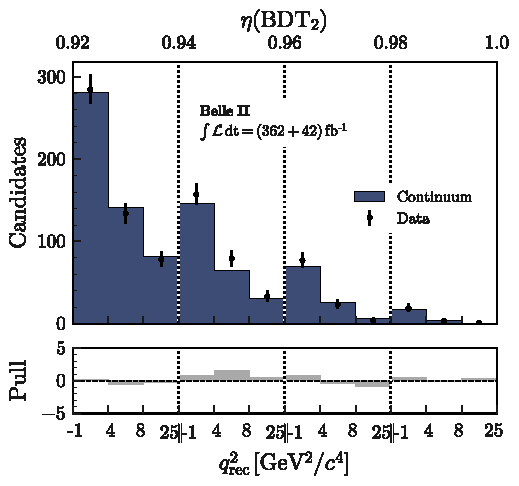
\includegraphics[width=\textwidth]{../plots/knunu-offres.pdf}
            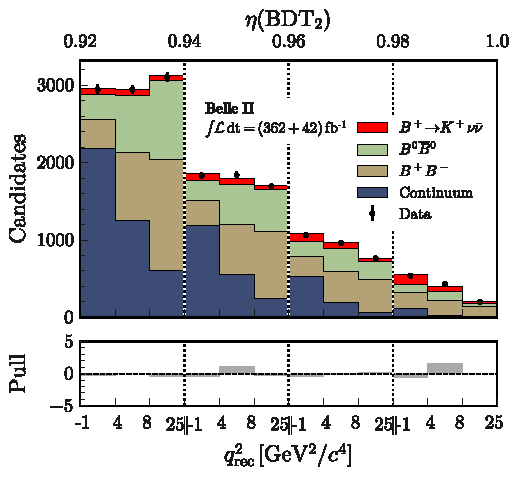
\includegraphics[width=\textwidth]{../plots/knunu-signal.pdf}
        \end{figure}
    \end{minipage}
    \end{frame}
    
\begin{frame}{Bayesian nuisance parameters}
    \begin{minipage}{0.6\textwidth}
        Priors can be defined using auxiliary data
        $$p(\nu|a) \propto p(a|\nu) p_0(\nu)$$
        %If $p_0(\nu)$ is chosen to have minimal impact, this overlaps with the frequentist treatment.
        
        Only in the Bayesian case, other prior choices are also allowed, e.g.
        $$ p(\nu) = \mathcal{N}(\nu | \nu_0, \sigma_\nu^2)$$
        
        % Bayesian approach also requires priors for POIs.
    \end{minipage}
    \begin{minipage}{0.39\textwidth}
        \begin{figure}
            \centering
            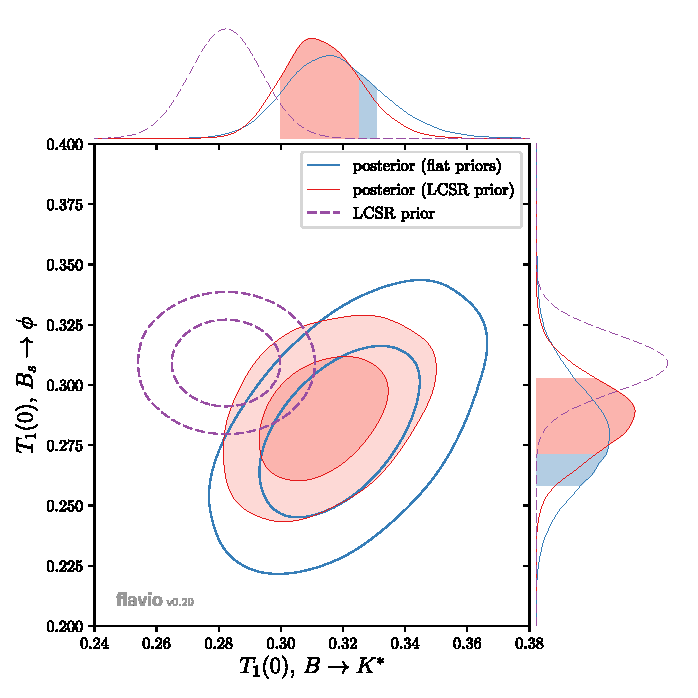
\includegraphics[width=\textwidth]{../plots/straub-posterior.pdf}
            \flushright \small
        \href{https://arxiv.org/pdf/2311.14647}{Paul 2017}
        \end{figure}
    \end{minipage}
\end{frame}
    
\begin{frame}{Bayesian updating}
        \vspace{-0.5cm}
        Can generally use measurements to \textit{update} our posterior
        $$
        p(\theta | x_1, x_2) = \frac{p(x_2|\theta)}{p(x_2)} p(\theta | x_1) = \frac{p(x_2|\theta)}{p(x_2)} \frac{p(x_1|\theta)}{p(x_1)} p(\theta).
        $$
        % Effectively what is done for combining measurement results (eg. \href{https://pdg.lbl.gov/}{PDG averages}).
        \begin{figure}
            \centering
            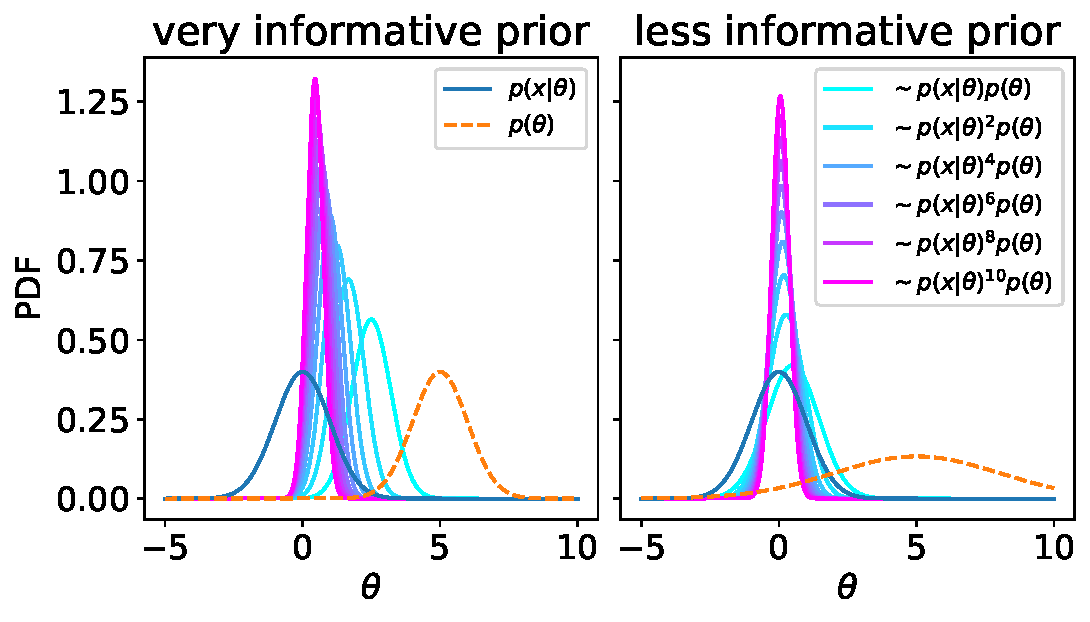
\includegraphics[width=0.65\linewidth]{../plots/updating.pdf}
        \end{figure}

        % A posterior based on all LHC data $x_{LHC}$
        % $$
        % p(\theta | x_{LHC}) = \frac{p(x_{LHC}|\theta)}{p(x_{LHC})} p(\theta)
        % $$
        % can be updated with LHC-HL data $x_{HL}$, with $p(\theta | x_{LHC})$ as a prior
        % $$
        % p(\theta | x_{LHC}, x_{HL}) = \frac{p(x_{HL}|\theta)}{p(x_{HL})} p(\theta | x_{LHC}) = \frac{p(x_{HL}|\theta)}{p(x_{HL})} \frac{p(x_{LHC}|\theta)}{p(x_{LHC})} p(\theta).
        % $$
        % Parameter values $\theta$ under which data $x_{LHC}, x_{HL}$ is more probable on average get weighted up, other values get weighted down.
\end{frame}

\begin{frame}{Bayesian updating in real life}
        \vspace{-0.5cm}
        PDFs for parameters are manifestly Bayesian.\\
        Combinations of $\mu_i \pm \sigma_i$ assume an underlying PDF for $\mu_i$.
        \begin{minipage}{0.44\textwidth}
            \begin{align*}
                \mathcal{R}(D) &= \frac{
                    \mathcal{B}(\bar B \to D \tau^- \bar{\nu}_\tau)
                }{
                    \mathcal{B}(\bar B \to D l^- \bar{\nu}_l)
                }\\
                \mathcal{R}(D^*) &= \frac{
                    \mathcal{B}(\bar B \to D^* \tau^- \bar{\nu}_\tau)
                }{
                    \mathcal{B}(\bar B \to D^* l^- \bar{\nu}_l)
                }
            \end{align*}
        \end{minipage}
        \begin{minipage}{0.55\textwidth}
            \begin{figure}
                \centering
                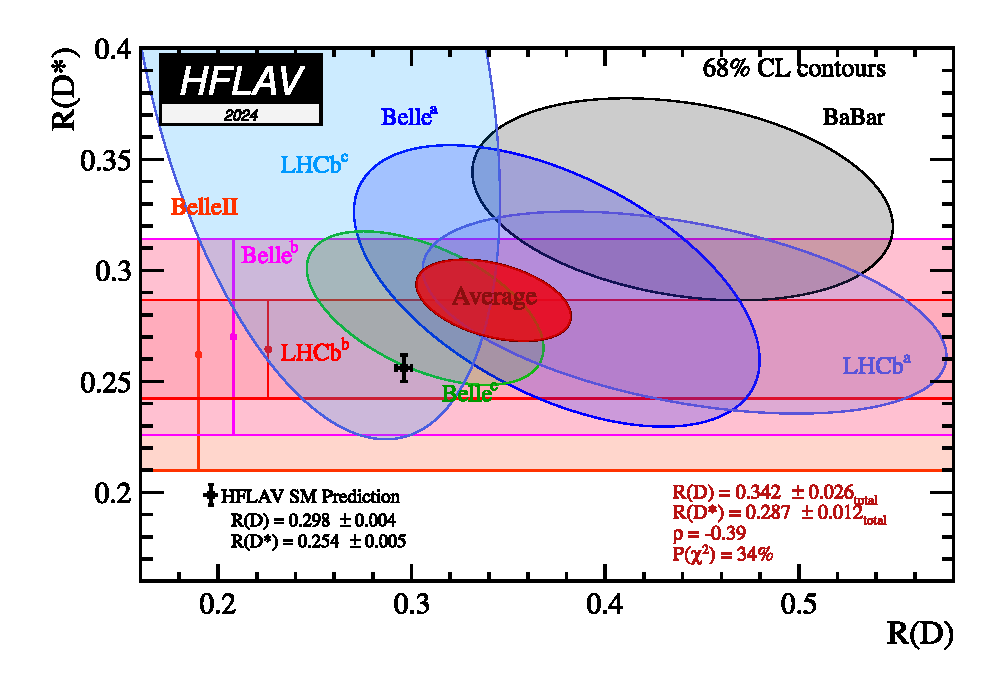
\includegraphics[width=\textwidth]{../plots/rd_rdstar.pdf}
            \end{figure}
        \end{minipage}
        \small Actual combinations a bit more involved \arrow \href{https://arxiv.org/pdf/2411.18639}{HFLAV 2024}.
\end{frame}

\begin{frame}{A simple linear model}
    \begin{figure}
        \centering
        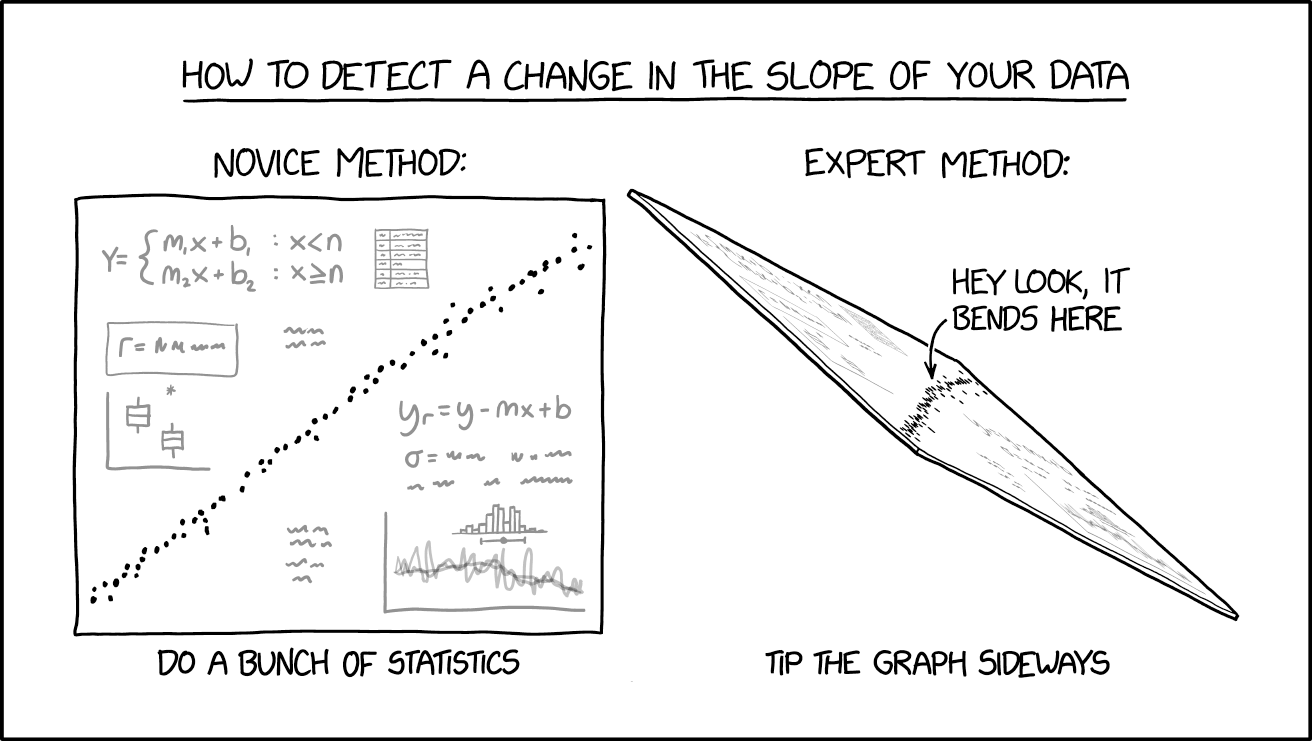
\includegraphics[width=0.8\linewidth]{../plots/change_in_slope_2x.png}
    \end{figure}
    % https://www.explainxkcd.com/wiki/images/9/9d/change_in_slope_2x.png
\end{frame}

\begin{frame}{A simple linear model}
    % https://www.pp.rhul.ac.uk/~cowan/stat/beijing10/cowan_beijing10_5.pdf
    % https://pdg.lbl.gov/2024/reviews/rpp2024-rev-statistics.pdf

    \begin{itemize}
        \item Our independent data : $\boldsymbol{X} = (x_i, y_i, \sigma_i)$
    \end{itemize}

    \begin{figure}
        \centering
        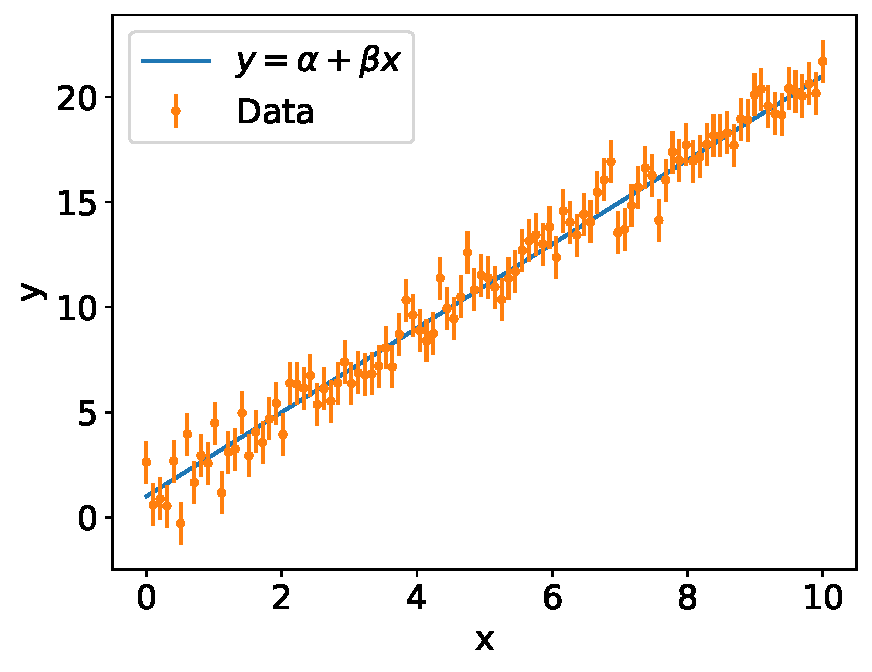
\includegraphics[width=0.5\linewidth]{../plots/linear_data.pdf}
    \end{figure}

\end{frame}

\begin{frame}{A simple linear model}
    \begin{itemize}
        \item Our independent data: $\boldsymbol{X} = (x_i, y_i, \sigma_i)$
        \item Our model:
        $$ p(\boldsymbol{X}|\theta_0, \theta_1) = \prod_{x_i, y_i,\sigma_i \in \boldsymbol{X}}\mathcal{N}(y_i | \mu(x_i|\theta_0, \theta_1), \sigma_i^2)$$
        $$\mu(x_i|\theta_0, \theta_1) = \theta_0 + \theta_1 x_i$$
         \item[\arrow] We want to know about $\theta_0$, do not care about $\theta_1$.
    \end{itemize}
\end{frame}

\begin{frame}{Unconstrained likelihood}
\vspace{-1cm}
    $$ -2\log p(\boldsymbol{X}|\theta_0, \theta_1) = \sum_{x_i, y_i,\sigma_i \in \boldsymbol{X}}\frac{\left(y_i -\mu(x_i|\theta_0, \theta_1)\right)^2}{\sigma_i^2}$$
    \begin{figure}
        \centering
        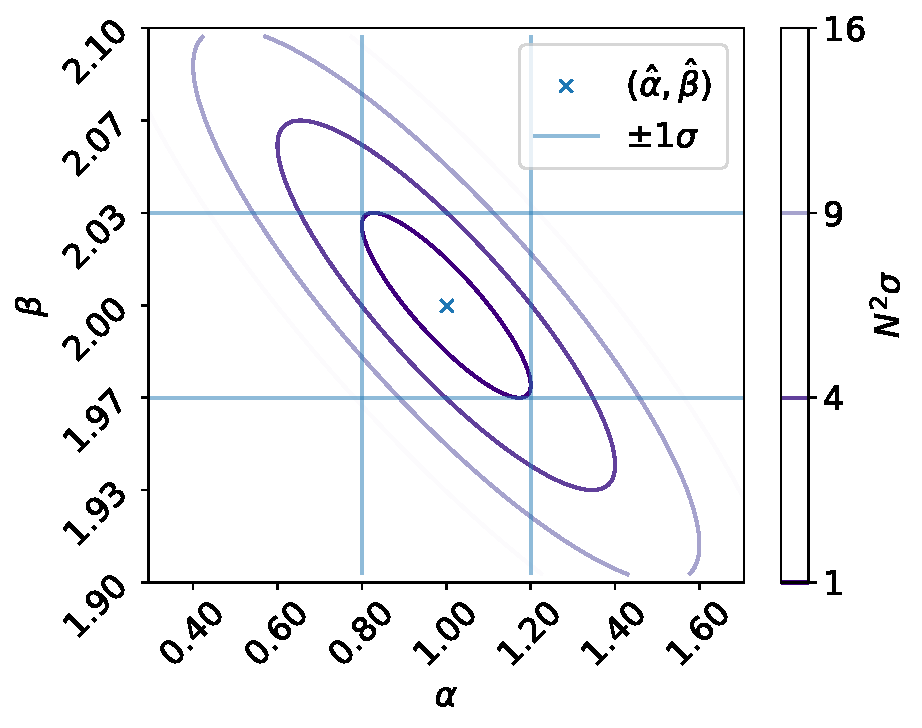
\includegraphics[width=0.5\linewidth]{../plots/nll_unconstr.pdf}
    \end{figure}
\end{frame}

\begin{frame}{Including a measurement of $\theta_1$: $t_1, \sigma_{t_1}$}
\vspace{-1cm}
    $$ -2\log p(\boldsymbol{X}|\theta_0, \theta_1) = \sum_{x_i, y_i,\sigma_i \in \boldsymbol{X}}\frac{\left(y_i -\mu(x_i|\theta_0, \theta_1)\right)^2}{\sigma_i^2} + \frac{\left(\theta_1 -t_1\right)^2}{\sigma_{t_1}^2} $$
    \begin{figure}
        \centering
        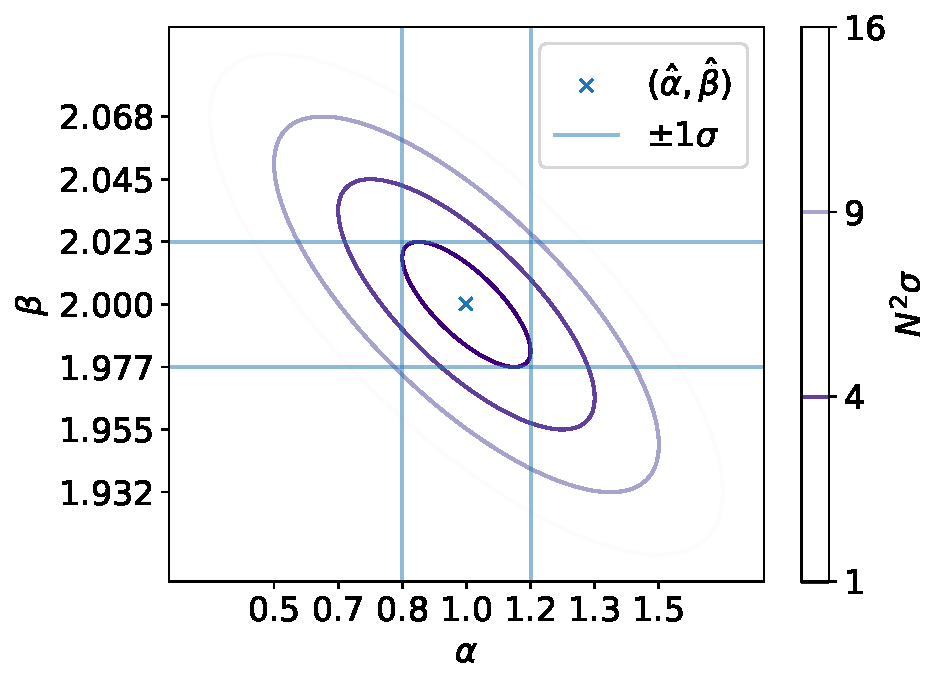
\includegraphics[width=0.5\linewidth]{../plots/nll_constr.pdf}
    \end{figure}
\end{frame}

\begin{frame}{Posterior}
\vspace{-1cm}
    $$p(\theta_0, \theta_1|\boldsymbol{X}) \propto p(\boldsymbol{X}|\theta_0, \theta_1) p(\theta_0)p(\theta_1)$$
    \begin{minipage}{0.4\linewidth}
        $$p(\theta_0) = \text{Uniform}(0,2)$$
        $$p(\theta_1) = \mathcal{N}(\theta_1 | t_1, \sigma_{t_1}^2)$$
    \end{minipage}
    \begin{minipage}{0.59\linewidth}
    \begin{figure}
        \centering
        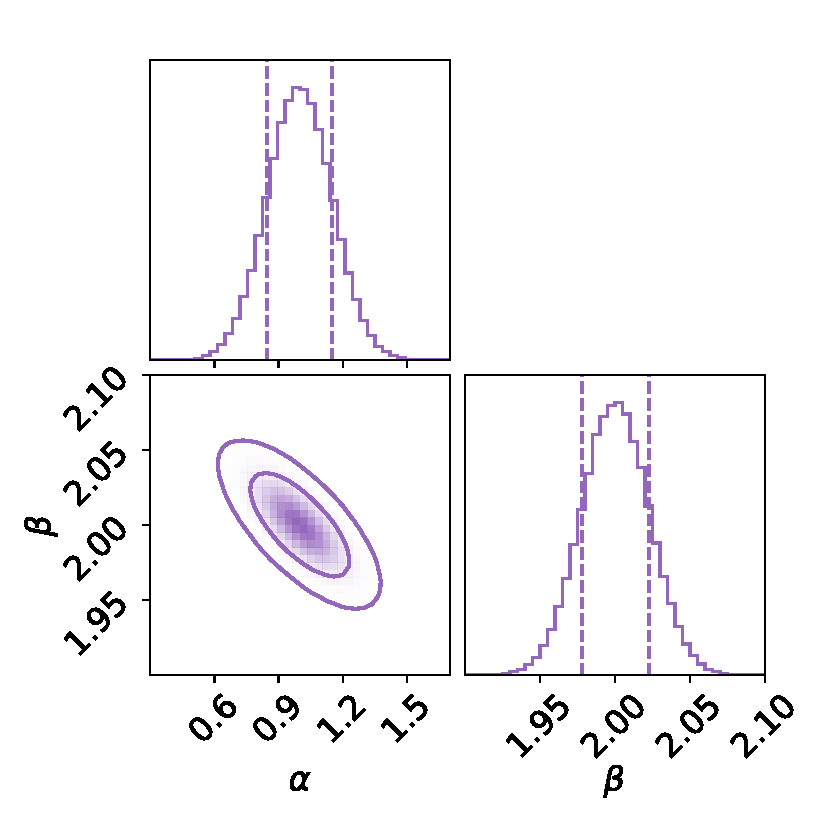
\includegraphics[width=0.8\linewidth]{../plots/posterior.pdf}
    \end{figure}
    \end{minipage}
\end{frame}

\begin{frame}{Marginal posterior}
\vspace{-1cm}
    $$p(\theta_0|\boldsymbol{X}) = \int d\theta_1 ~ p(\theta_0, \theta_1|\boldsymbol{X}) = \mathcal{N}(\theta_0 | \theta_0^*, \sigma_{\theta_0})$$
    \begin{minipage}{0.4\linewidth}
    In this example, we get
        \begin{itemize}
            \item $\theta_0^* = \hat \theta_0$
            % $$
            % \hat \theta_0 =
            % $$
            \item 68\% HDI = $\hat \theta_0 \pm \sigma_{\theta_0}$
            % $$
            % \sigma_{\theta_0}^2 = \sum_{x_i,  \sigma_i\in \boldsymbol{x}, \boldsymbol{\sigma}}\sigma_{t_1}x_i^2 + \sigma_i^2
            % $$
        \end{itemize}
    \end{minipage}
    \begin{minipage}{0.59\linewidth}
    \begin{figure}
        \centering
        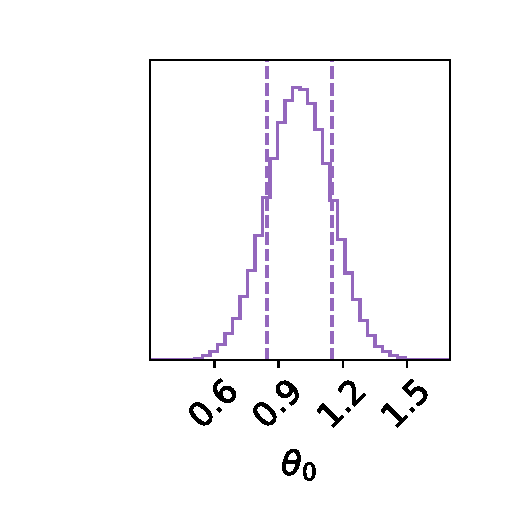
\includegraphics[width=0.7\linewidth]{../plots/marginal_posterior.pdf}
    \end{figure}
    \end{minipage}
\end{frame}

\begin{frame}
\center
\Large
MCMC
\end{frame}

\begin{frame}{The hard part ...}
\begin{itemize}
    \item We only want the posterior for $\theta$ alone.
    \item Remove nuisance parameters by integrating over $\nu$.
    \item[\arrow] The \textit{marginal posterior} is
        $$
        p(\theta | x) = \int d\nu ~ p(\psi, \nu | x)
        $$
    \item Commonly a high dimensional integral\\ \arrow compute with Monte Carlo methods.
\end{itemize}
\end{frame}

\begin{frame}{Markov chain}
    A sequence of events, where probability of the next state depends solely on the current state
    $$
    \ldots \to \theta_{i} \sim g(\theta_{i} | \theta_{i-1}) \to \theta_{i+1} \sim g(\theta_{i+1} | \theta_{i}) \to \ldots
    $$
    for some \textit{proposal distribution} $g$. 
\end{frame}

\begin{frame}{Markov Chain Monte Carlo (MCMC)}
    \begin{figure}
        \centering
        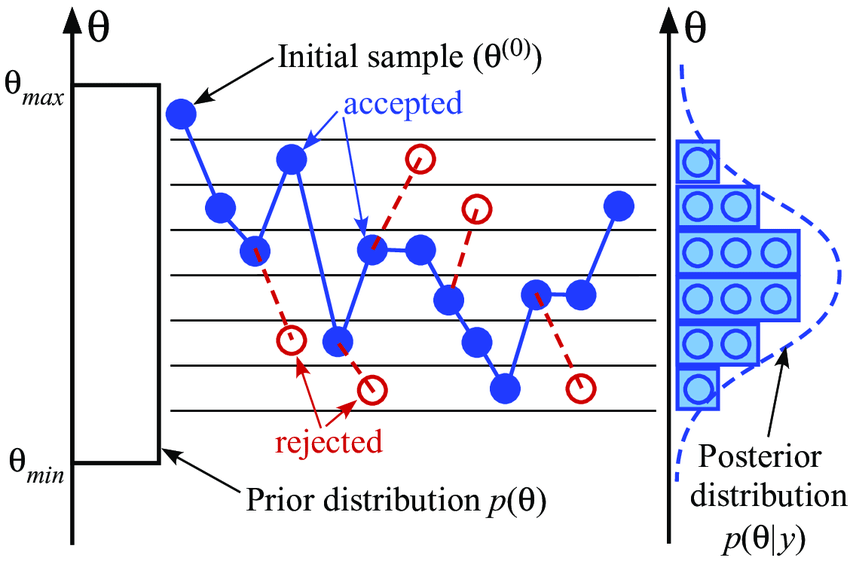
\includegraphics[width=0.6\linewidth]{../plots/mcmc_diagram.png}
    \end{figure}
    % https://doi.org/10.3390/app10010272
\end{frame}

\begin{frame}{Metropolis-Hastings}
We loop
\begin{enumerate}
    \item Generate $\theta \sim g(\theta|\theta_i)$
    \item Update
    \begin{equation*}
        \theta_{i+1} =
        \begin{cases}
            \theta  &\quad u \leq \text{min}\left(1, \frac{p(\theta)g(\theta|\theta_i)}{p(\theta_i)g(\theta_i|\theta)}\right)\\
            \theta_i &\quad \text{otherwise}
        \end{cases}
    \end{equation*}
    where $u \sim \text{Uniform}(0, 1)$
\end{enumerate}
\textit{Note}: Need to define a proposal distribution $g(\theta|\theta_0)$.
\end{frame}

\begin{frame}{Chains}
    In MCMC we generate a sequence
    $$
    \theta_0 \to \theta_1 \to \theta_2 \to \ldots
    $$
    \begin{minipage}{0.49\textwidth}
        Only one start can land you in local minima.
        \begin{align*}
            &\theta_0^0 \to \theta_1^0 \to \theta_2^0 \to \ldots \\
            &\theta_0^1 \to \theta_1^1 \to \theta_2^1 \to \ldots \\
            &\theta_0^2 \to \theta_1^2 \to \theta_2^2 \to \ldots \\
            &\ldots
        \end{align*}
    \end{minipage}
    \begin{minipage}{0.49\textwidth}
        \begin{figure}
            \centering
            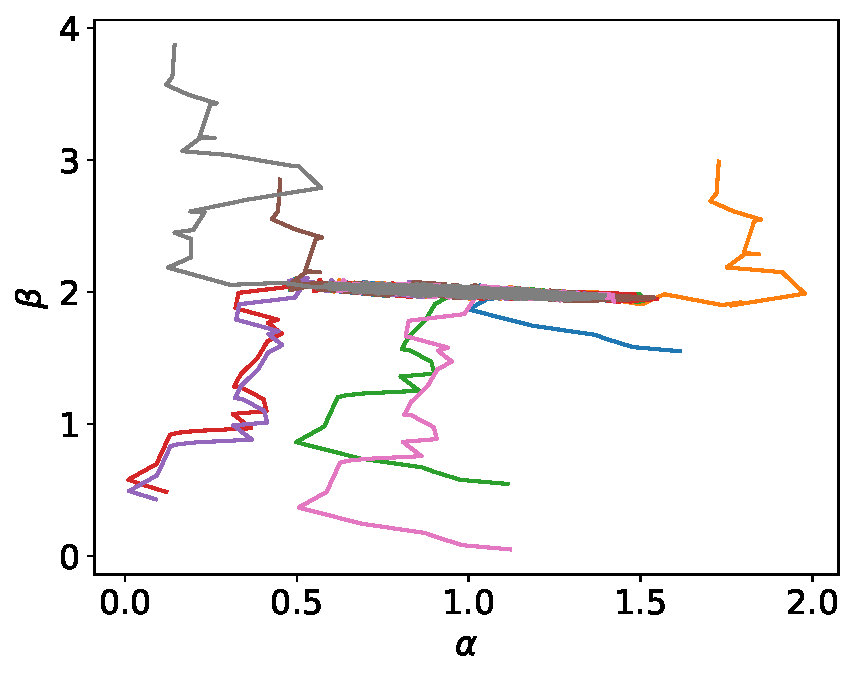
\includegraphics[width=0.9\textwidth]{../plots/chain_walk.pdf}
        \end{figure}
    \end{minipage}

\end{frame}

\begin{frame}{Convergence}
    Trace plots are a useful convergence diagnostic
    \begin{minipage}[t]{0.49\linewidth}
    \begin{figure}
        \centering
        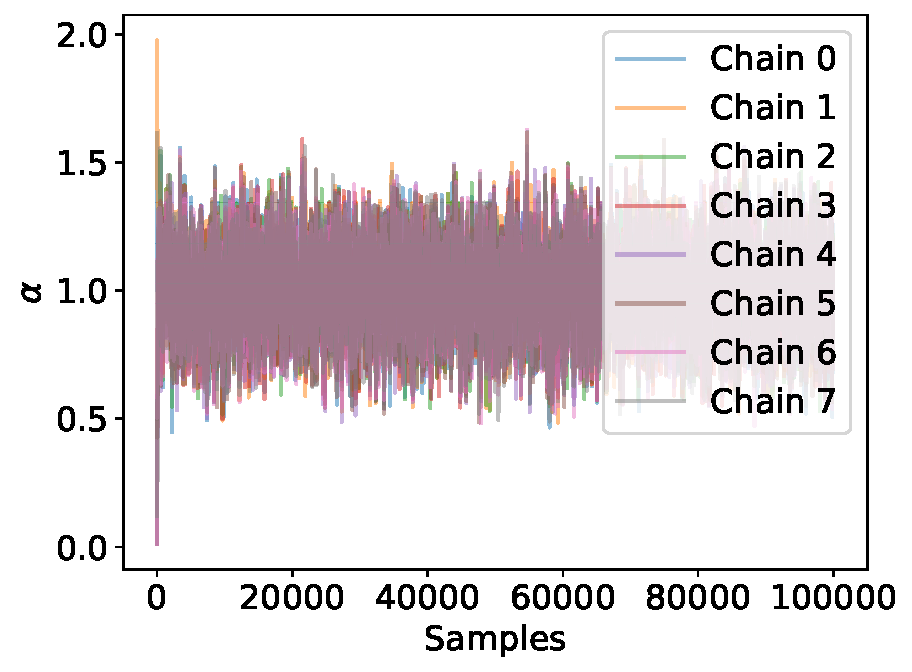
\includegraphics[width=\linewidth]{../plots/trace_theta0.pdf}
    \end{figure}
    \end{minipage}
    \begin{minipage}[t]{0.49\linewidth}
    \begin{figure}
        \centering
        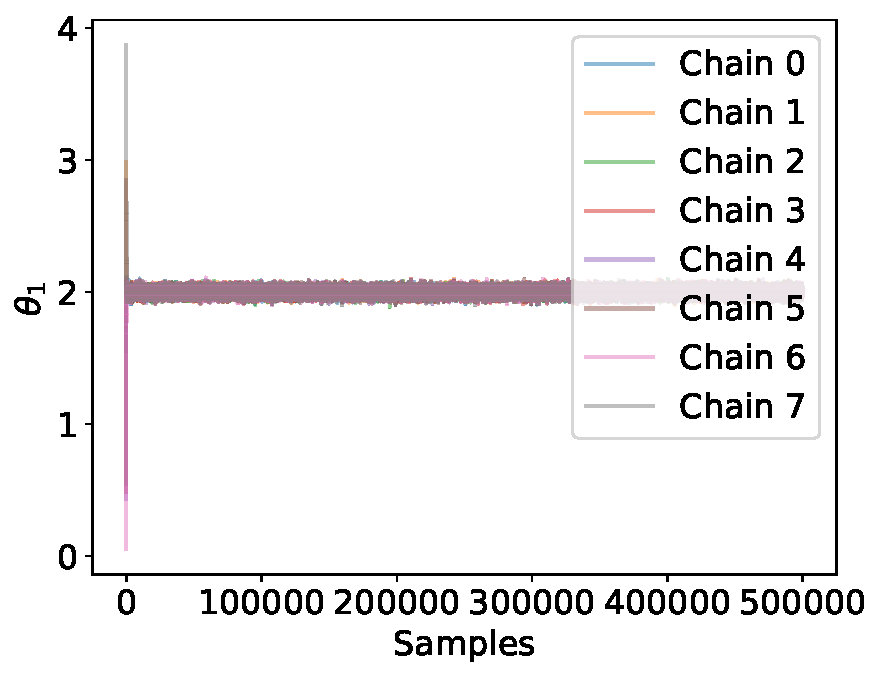
\includegraphics[width=\linewidth]{../plots/trace_theta1.pdf}
    \end{figure}
    \end{minipage}
    ... but one can become more fancy. %TODO reference
\end{frame}

\begin{frame}
    \center
    \Large
    Model comparison
\end{frame}

\begin{frame}{Point-wise: P-values}
    \vspace{-1cm}
    $$
    P(\lambda_{obs}|M_0) = \int_{\lambda_{obs}}^\infty d\lambda ~ p(\lambda|M_0), \quad  \lambda = -2 \ln \frac{p(x|\theta, M_0)}{p(x|\theta, M_1)} ~^\dagger
    $$
    \begin{figure}
        \centering
        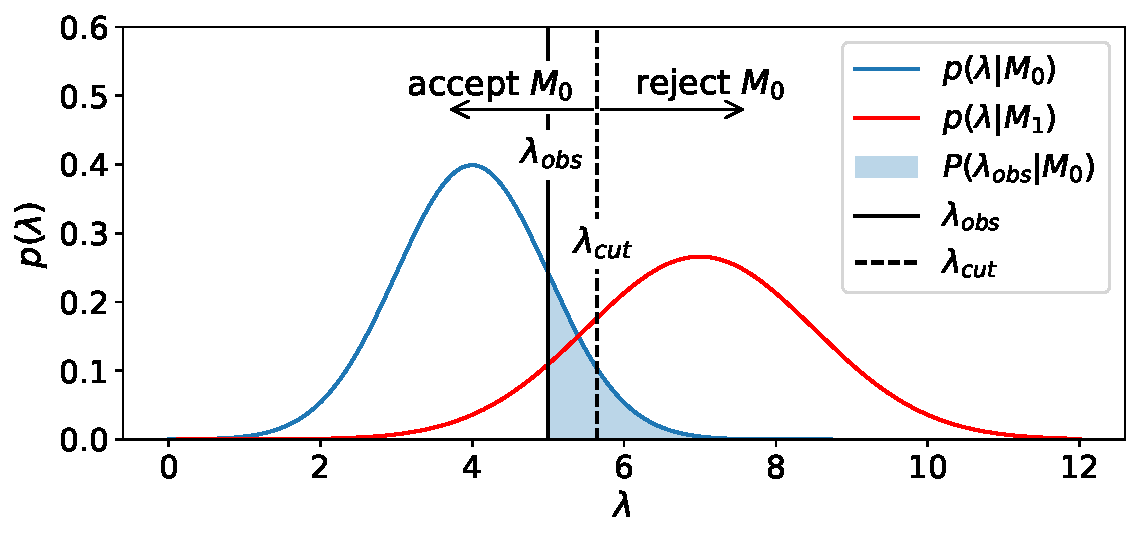
\includegraphics[width=0.65\textwidth]{../plots/hypo.pdf}
    \end{figure}
    \small
    $^\dagger$ Likelihood ratio = optimal test statistic \arrow Newman-Pearson lemma
\end{frame}

\begin{frame}{Averaged: Bayes factor}
    \vspace{-0.5cm}
        \begin{minipage}{0.74\textwidth}
            Compare the probabilities of the observed data being produced by a given model.
            \begin{align*}
                p(\theta | x, M) &= \frac{p(x | \theta, M) ~ p(\theta | M)}{\textcolor{red}{p(x | M)}}\\
                \textcolor{red}{p(x | M)} &= \int d^n \theta ~ p(x | \theta, M) ~ p(\theta | M)\\
                B &= \frac{p(x | M_1)}{p(x| M_0)}
            \end{align*}
        \end{minipage}
        \begin{minipage}{0.25\textwidth}
            \begin{figure}
                \centering
                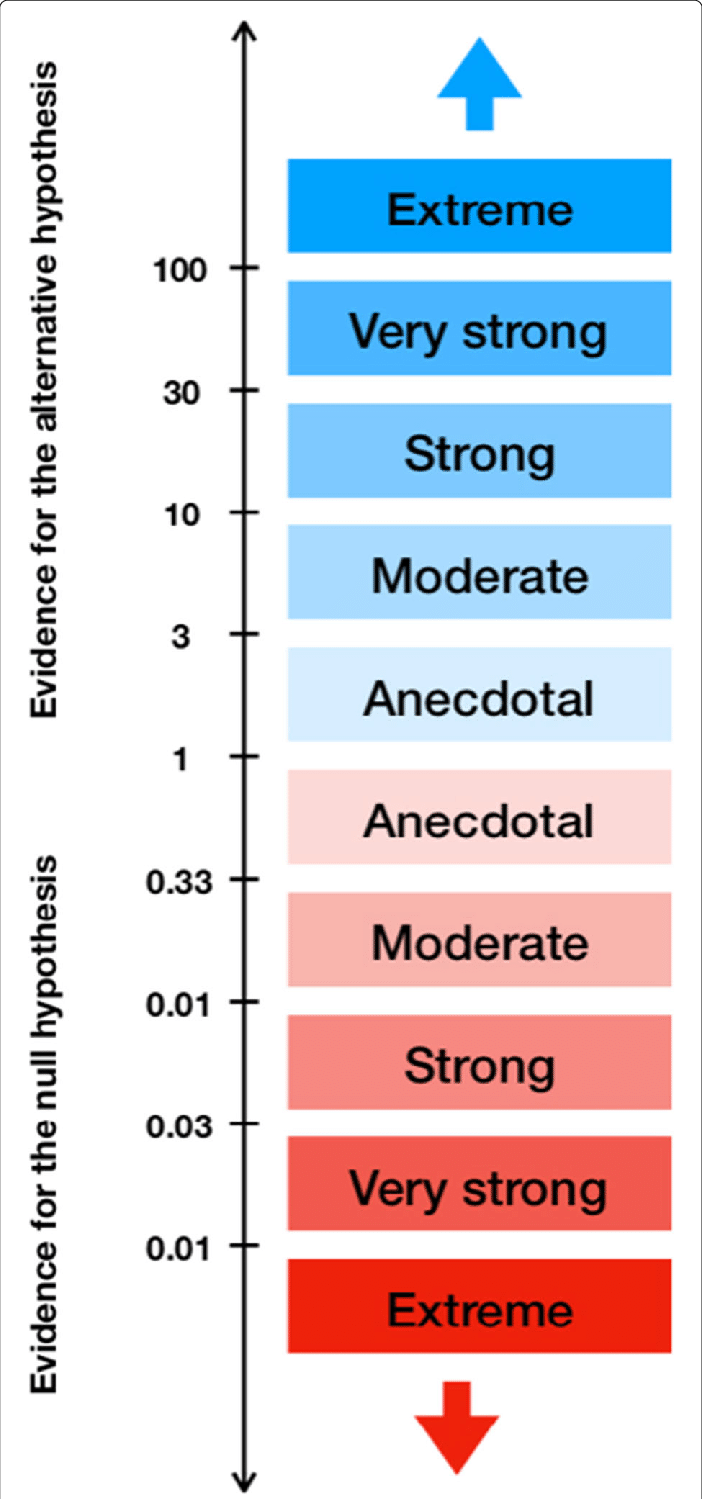
\includegraphics[width=\textwidth]{../plots/jeffreys-scale.png}
                %https://www.researchgate.net/publication/341958289/figure/fig1/AS:902030868615168@1592072326255/JASP-classification-scheme-for-the-Bayes-factor-BF-10.png
            \end{figure}
        \end{minipage}
    \end{frame}

\begin{frame}{$b\to u l^- \bar \nu$ in the Weak Effective Theory}
    \begin{figure}
        \centering
        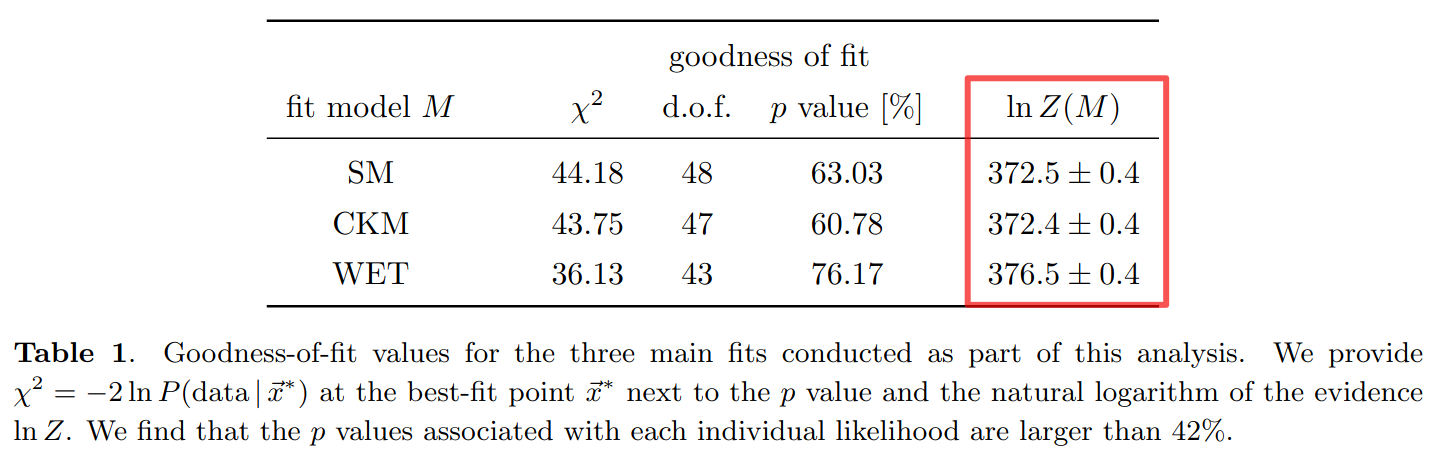
\includegraphics[width=\textwidth]{../plots/wet-bayes.png}
    \end{figure}
    $$
    B = \exp(\ln Z(WET) - \ln Z (SM)) = 54.6
    $$
    \begin{flushright}
        \href{https://arxiv.org/pdf/2302.05268}{arXiv:2302.05268v2 [hep-ph]}
    \end{flushright}
\end{frame}

\begin{frame}{Tools to try}
\begin{figure}
    \center
    \href{
        https://github.com/bat
    }{
\includegraphics[width=0.3\textwidth]{../plots/bat.pdf}}
    \hfill
    \href{
        https://www.pymc.io/
    }{
\includegraphics[width=0.35\textwidth]{../plots/pymc.png}}
    \hfill
    \href{
        https://python.arviz.org/en/stable/
    }{
\includegraphics[width=0.3\textwidth]{../plots/arviz.png}}
\end{figure}
\end{frame}

% \begin{frame}{Exercises}

% \textbf{a simple MCMC algorithm}\\

% \end{frame}

% \begin{frame}{Exercises: s+b problem}
% \small
% You do a binned analysis. You observe [155, 121,  13] in each bin respectively. From simulation, you expect to see [90, 30, 0] signal events (where the last bin acts as a control measurement) and [50, 70, 10] background events.\\
% Hint: It is better to work with log-probabilities
% \end{frame}

% \begin{frame}{Exercises: s+b problem}
% \small
% \begin{itemize}
%     \item Construct a likelihood function (chi2)
%     \item What is the best fit point?
%     \item What are the frequentist limits?
%     \item What would a sensible choice of priors be for this example?
%     \item Use an implementation of the Metropolis Hastings algorithm to sample from the posterior
%     \item Make a corner plot of the posterior
%     \item How do the mode of the posterior and the credible intervals compare to the best fit point and frequentist limits?
% \end{itemize}
% \end{frame}

%%%%%%%%%%%%%%%%%%%%%%%%%%%%%%%%%%%%%%%%%%%%%%%%%%%%%%%%%%%%%%%%%%%%%%%%%%%%%%%%%%%
\appendix




\end{document}


% https://drive.google.com/drive/folders/16CIMfhQkyEqMYkhLcsnzN0Yu5C2WHNU74

% https://pdg.lbl.gov/2024/reviews/rpp2024-rev-statistics.pdf

interested in using a given sample of data to make inferences about a probabilistic model

In Bayesian statistics, the subjective interpretation of probability is used to quantify one’s
degree of belief in a hypothesis. This allows one to define a probability density function (p.d.f.) for
a parameter, which reflects one’s knowledge about where its true value lies.

 hypothesis H is a statement about the probability for the data,
often written P (x|H)

If the probability P (x|H) for data x is regarded as a function of the hypothesis H, then it is
called the likelihood of H, usually written L(H). Often the hypothesis is characterized by one or
more parameters θ, in which case L(θ) = P (x|θ) is called the likelihood function.

In the Bayesian approach, inference is based on the posterior probability for H given the data
x, which represents one’s degree of belief that H is true given the data. 

Bayesian statistics supplies no unique rule for determining the prior.  it is important to carry out a sensitivity analysis, that is, to show how the result changes under a reasonable variation of the prior probabilities

For the special case of a constant prior, one can see from Bayes’ theorem (40.37) that the
posterior is proportional to the likelihood, and therefore the mode (peak position) of the posterior
is equal to the maximum-likelihood estimator. The posterior mode, however, will change in general
upon a transformation of parameter. One may use as the Bayesian estimator a summary statistic
other than the mode, such as the median, which is invariant under parameter transformation. But
this will not in general coincide with the MLE